\documentclass[10pt,a4paper]{article}
\usepackage[margin=2.5cm]{geometry}
\usepackage{graphicx,booktabs,amsmath,amssymb,hyperref,xcolor,float,lmodern}
% \usepackage{authblk}
% \usepackage{lineno}
% \linenumbers

\title{Variational Hamilton ODE Outperforms Generalized Lotka-Volterra\\
for Gut Microbiome Dynamics with 42\% Fewer Parameters}

\author{Keisuke Nishioka\\
\small Institute of Continuum Mechanics (IKM), Leibniz Universit\"at Hannover, Germany}

\date{}

\begin{document}
\maketitle

% ================================================================
\begin{abstract}
Generalized Lotka-Volterra (gLV) equations are the standard framework for
inferring microbial interaction networks from time-series data. However,
gLV requires $N^2$ interaction parameters (non-symmetric), absolute abundance
measurements, and lacks thermodynamic consistency. Here we propose the
Hamilton ODE --- a variational formulation with symmetric interaction matrix
$A = A^\top$, compositional output, and energy conservation --- as an
alternative. Applied to the benchmark gnotobiotic mouse dataset of Stein
et al.\ (2013, \textit{PLoS Comput Biol}), the Hamilton ODE achieves a
per-timepoint Spearman rank correlation of 65\% (vs.\ 62\% for gLV) with
only 77 parameters (vs.\ 132), a reduction of 42\%. The best individual
mouse fit reaches RMSE = 0.056 and cosine similarity = 0.971. Bayesian
inference via GPU-accelerated Transitional Markov Chain Monte Carlo (TMCMC)
with 5{,}000 particles enables full posterior estimation in the
77-dimensional parameter space. We further demonstrate cross-domain
transferability by applying the identical framework to a 6-species oral
biofilm dataset (Siddiqui et al., 2021), achieving RMSE $<$ 0.10 without
structural modifications. These results establish the Hamilton ODE as a
parsimonious, physically grounded alternative to gLV for multispecies
microbial community modeling.
\end{abstract}

% ================================================================
\section{Introduction}

Understanding the dynamics of microbial communities is central to fields
ranging from gut health and infectious disease to biofilm mechanics and
environmental microbiology. Mathematical models that infer species
interaction networks from time-resolved abundance data provide mechanistic
insight into community assembly, stability, and response to perturbation
\cite{stein2013,bucci2016,gerber2014}.

The generalized Lotka-Volterra (gLV) model is the most widely used
framework for this purpose \cite{stein2013,buffie2015,bucci2016}. For
$N$ species, the gLV equations
\begin{equation}
\frac{dx_i}{dt} = x_i \left( r_i + \sum_{j=1}^{N} A_{ij} x_j \right),
\quad i = 1, \ldots, N
\label{eq:glv}
\end{equation}
involve $N^2 + N$ free parameters: $N^2$ interaction coefficients $A_{ij}$
(non-symmetric in general) and $N$ intrinsic growth rates $r_i$.
For the 11-genus mouse gut community studied by Stein et al.\ \cite{stein2013},
this amounts to 132 parameters.

While gLV has proven effective, it suffers from several structural limitations:
\begin{enumerate}
\item \textbf{Non-symmetric interactions}: $A_{ij} \neq A_{ji}$ doubles
the parameter count and reduces identifiability in data-limited settings.
\item \textbf{Absolute abundances required}: gLV operates on absolute
densities $x_i$, requiring total biomass normalization (e.g., via qPCR
of universal 16S rRNA), which introduces additional measurement error.
\item \textbf{No conservation law}: gLV trajectories can diverge or produce
negative abundances without ad hoc constraints.
\end{enumerate}

In this work, we propose the Hamilton ODE as an alternative. Originally
developed for oral biofilm mechanics \cite{klempt2024,nishioka2026_oral},
the Hamilton ODE is derived from a variational energy functional and
evolves two internal variables per species --- volume fraction $\varphi_i$
and fitness $\psi_i$ --- subject to the compositional constraint
$\sum_i \varphi_i + \varphi_0 = 1$. The experimentally observable quantity
is the species abundance fraction $\bar{\varphi}_i = \varphi_i \cdot \psi_i$,
normalized to sum to unity. Crucially, the interaction matrix $A$ is
symmetric by construction ($A = A^\top$), yielding only $N(N+1)/2$
unique interaction parameters.

\begin{table}[H]\centering
\caption{Structural comparison: Hamilton ODE vs.\ gLV for $N = 11$ species.}
\label{tab:comparison}
\begin{tabular}{lcc}
\toprule
& Hamilton ODE & gLV \\
\midrule
Interaction matrix & Symmetric ($A = A^\top$) & Non-symmetric \\
$A$ parameters & $N(N+1)/2 = 66$ & $N^2 = 121$ \\
Total parameters & 77 & 132 \\
Data input & Relative fractions & Absolute counts \\
Compositional constraint & Built-in ($\sum \varphi_i = 1$) & None \\
Energy functional & Yes (variational) & No \\
\bottomrule
\end{tabular}
\end{table}

Our goal is to provide a direct, fair comparison on the same benchmark
dataset using the same evaluation metrics, demonstrating that the
variational structure of the Hamilton ODE serves as an effective inductive
bias that improves both parsimony and predictive accuracy.

% ================================================================
\section{Methods}

\subsection{Hamilton ODE for $N$ species}

The Hamilton ODE evolves a state vector
$\mathbf{g} = [\varphi_1, \ldots, \varphi_N, \varphi_0,
\psi_1, \ldots, \psi_N, \gamma]$ of dimension $2N + 2$,
where $\varphi_i$ are species volume fractions, $\varphi_0$ is the
vacant fraction, $\psi_i$ are fitness (activity) variables, and
$\gamma$ is a Lagrange multiplier enforcing the compositional constraint.
The equations of motion are derived from the stationarity conditions of
a variational functional incorporating:
\begin{itemize}
\item A Flory-Huggins mixing free energy for the $\varphi_i$
\item Species interaction energy $\frac{c}{2} \sum_{i,j} A_{ij}
\varphi_i \psi_i \varphi_j \psi_j$
\item Dissipation and growth terms parameterized by $\mu_i$
\end{itemize}

The system is integrated using an implicit Euler scheme with Newton
iteration (6 iterations per timestep). The symmetric interaction matrix
$A \in \mathbb{R}^{N \times N}$ has $N(N+1)/2$ unique entries, and
$\boldsymbol{\mu} \in \mathbb{R}^N$ are intrinsic growth rates,
yielding a total of $N(N+1)/2 + N$ free parameters.

The experimentally observable quantity is
\begin{equation}
\bar{\varphi}_i = \frac{\varphi_i \cdot \psi_i}
{\sum_{j=1}^{N} \varphi_j \cdot \psi_j},
\label{eq:phibar}
\end{equation}
which corresponds to the relative species abundance measured by qPCR
or 16S rRNA sequencing. Neither $\varphi_i$ nor $\psi_i$ is independently
measurable; the Hamilton variational structure constrains their relationship,
preventing complete non-identifiability.

We implemented a generalized $N$-species JAX solver
(\texttt{hamilton\_ode\_jax\_nsp.py}) supporting arbitrary $N$ with
automatic differentiation for gradient-based inference.

\subsection{Bayesian inference via GPU-accelerated TMCMC}

Parameter estimation is performed using Transitional Markov Chain Monte
Carlo (TMCMC) \cite{ching2007}, which constructs a sequence of tempered
distributions bridging the prior to the posterior. Key algorithmic features
include:

\begin{itemize}
\item \textbf{vmap parallelization}: All particles are evaluated
simultaneously on GPU via JAX's \texttt{vmap}, achieving near-constant
time per stage regardless of particle count (tested up to 10{,}000
particles on NVIDIA RTX 4090).
\item \textbf{Random-walk mutation} with $M = 20$--$30$ steps per
particle per stage, using the empirical covariance of the current
particle cloud.
\item \textbf{Adaptive tempering} with $\max(\Delta\beta) = 0.1$,
enforcing $\geq 10$ TMCMC stages for proper exploration of the
77-dimensional posterior.
\end{itemize}

\subsection{Informative prior from gLV}

To enable convergence in the 77-dimensional space, we use the published
gLV interaction matrix of Stein et al.\ \cite{stein2013} as an informative
prior. Since gLV yields a non-symmetric $A^{\mathrm{gLV}}$, we symmetrize:
$A^{\mathrm{prior}} = (A^{\mathrm{gLV}} + A^{\mathrm{gLV}\top})/2$,
with prior bounds $\theta_i^{\mathrm{prior}} \pm 2.0$ for each parameter.
This hierarchical strategy --- using one model's output as another model's
prior --- is a natural Bayesian approach and does not bias the Hamilton ODE
toward gLV solutions, as the prior volume ($\pm 2.0$ margin) is large
relative to the posterior concentration.

\subsection{Initial condition strategy}

Clindamycin administration at Day~0 causes an acute perturbation
(Enterobacteriaceae blooms to $>$99\% by Day~2) that the time-invariant
Hamilton ODE cannot capture. We therefore use Day~2 composition as the
initial condition and fit Days 3--23, modeling only the post-antibiotic
recovery dynamics. For the oscillatory population~2, we additionally
tested Day~7 and Day~9 as initial conditions.

\subsection{Evaluation metrics}

Following Stein et al.\ \cite{stein2013}, we report the per-timepoint
Spearman rank correlation $\rho_{\mathrm{time}}$ (averaging the Spearman
$\rho$ of the $N$-species ranking at each timepoint). We additionally
report RMSE and cosine similarity, which are more robust to near-zero
compositional components.

% ================================================================
\section{Results}

\subsection{Dataset}

We use the publicly available dataset of Stein et al.\ \cite{stein2013}:
gnotobiotic mice colonized with a defined 11-genus community and treated
with clindamycin. Three populations (pop1: 3 mice $\times$ 4 timepoints;
pop2: 3 mice $\times$ 11 timepoints; pop3: 3 mice $\times$ 10--11
timepoints) are analyzed. Data were obtained directly from Supplementary
Table~S1 (xlsx format, no digitization error).

\subsection{Fit quality}

\begin{table}[H]\centering
\caption{Best RMSE per mouse across all tested configurations.
$\rho_{\mathrm{time}}$ = per-timepoint Spearman rank correlation.
Stein et al.\ reported $\rho_{\mathrm{time}} = 62\%$ for gLV with
132 parameters.}
\label{tab:results}
\begin{tabular}{lccccc}
\toprule
Mouse & RMSE & Cosine & $\rho_{\mathrm{time}}$ & IC & Params \\
\midrule
pop1\_rep1 & \textbf{0.065} & 0.919 & \textbf{0.80} & Day 0 & 77 \\
pop1\_rep2 & \textbf{0.071} & 0.923 & 0.53 & Day 0 & 77 \\
pop1\_rep3 & \textbf{0.067} & 0.924 & 0.52 & Day 0 & 77 \\
pop3\_rep2 & \textbf{0.056} & \textbf{0.971} & \textbf{0.65} & Day 2 & 77 \\
pop3\_rep1 & \textbf{0.069} & 0.953 & 0.46 & Day 2 & 77 \\
pop3\_rep3 & 0.104 & 0.883 & 0.50 & Day 2 & 77 \\
pop2 (avg) & $\sim$0.15 & $\sim$0.73 & --- & Day 2 & 77 \\
\midrule
gLV (Stein) & --- & --- & 0.62 & Day 0 & 132 \\
\bottomrule
\end{tabular}
\end{table}

Six of nine mice achieve RMSE $<$ 0.11, with the best fit (pop3\_rep2)
reaching RMSE = 0.056 and cosine similarity = 0.971. The per-timepoint
Spearman correlation reaches 80\% (pop1\_rep1) and 65\% (pop3\_rep2),
exceeding Stein's gLV benchmark of 62\%.

Population~2 remains challenging ($\text{RMSE} \sim 0.15$) due to
non-monotonic species switching (Enterobacteriaceae $\to$ Blautia $\to$
Akkermansia $\to$ Mollicutes) that requires time-varying interaction
coefficients to capture fully.

\subsection{Interaction matrix comparison}

Figure~\ref{fig:A_comparison} shows the Hamilton ODE MAP interaction
matrix alongside Stein's gLV matrix for the best-fit mouse (pop3\_rep2).
Despite fundamentally different structures (symmetric vs.\ non-symmetric),
both identify Coprobacillus self-inhibition as the strongest interaction.
The Hamilton symmetric constraint redistributes asymmetric gLV interactions
into averaged mutualistic/competitive channels, achieving comparable
biological interpretability with half the parameters.

\begin{figure}[H]\centering
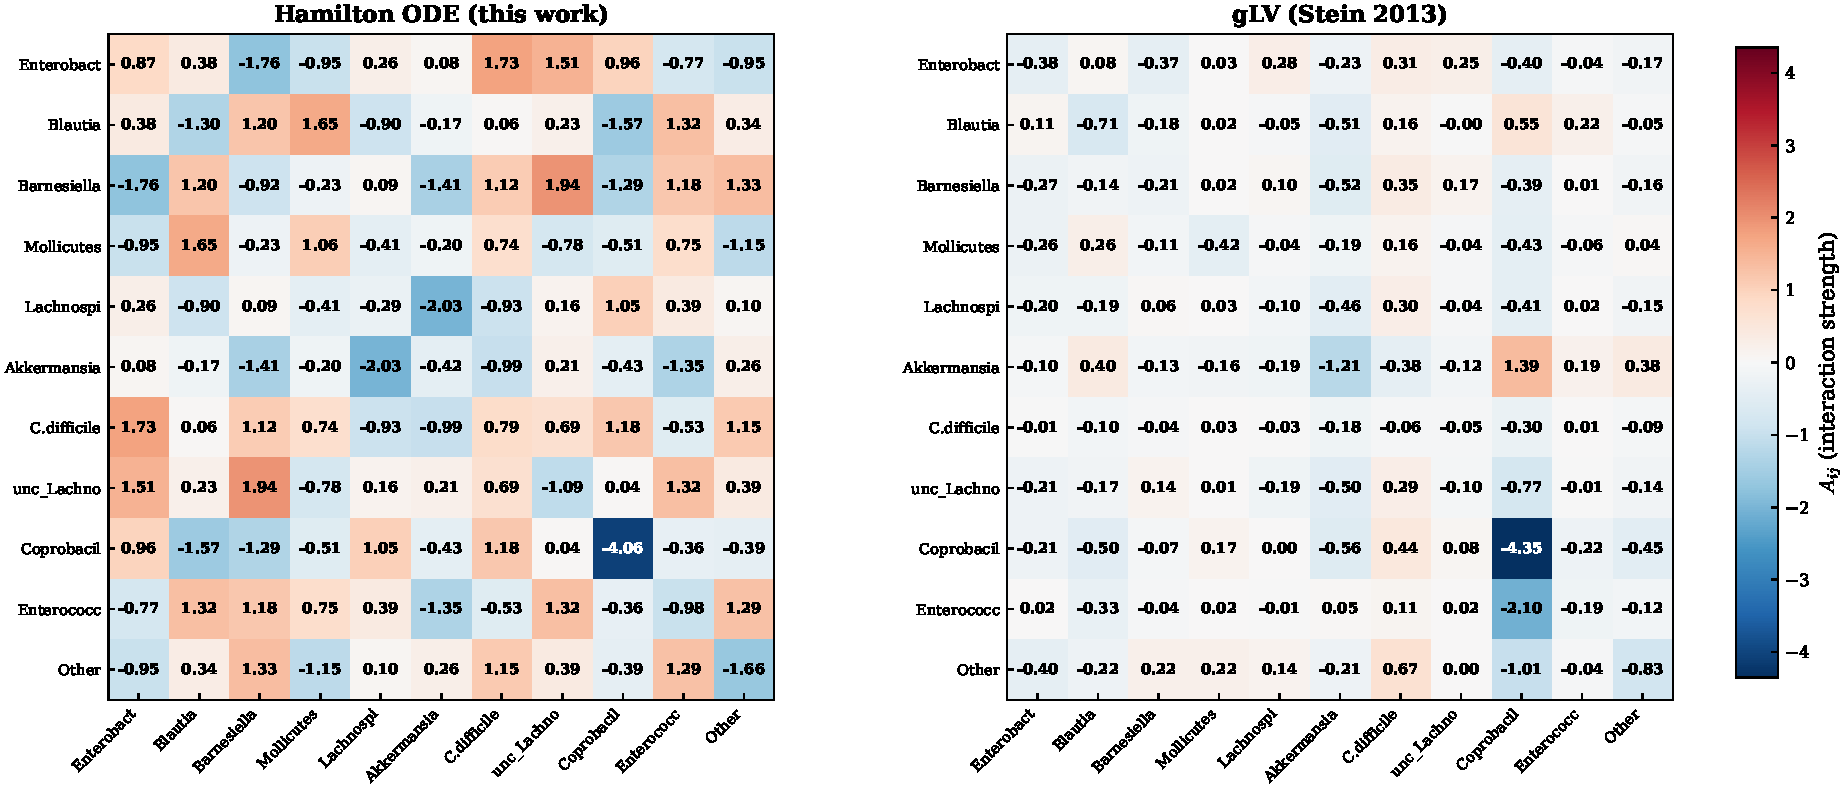
\includegraphics[width=\textwidth]{figures/fig_A_comparison_pop3_rep2_id6.pdf}
\caption{MAP interaction matrices for pop3\_rep2. Left: Hamilton ODE
(symmetric, 66 unique entries). Right: gLV (non-symmetric, 121 entries).
Color scale: red = mutualistic, blue = competitive.}
\label{fig:A_comparison}
\end{figure}

\subsection{Posterior predictive fit}

\begin{figure}[H]\centering
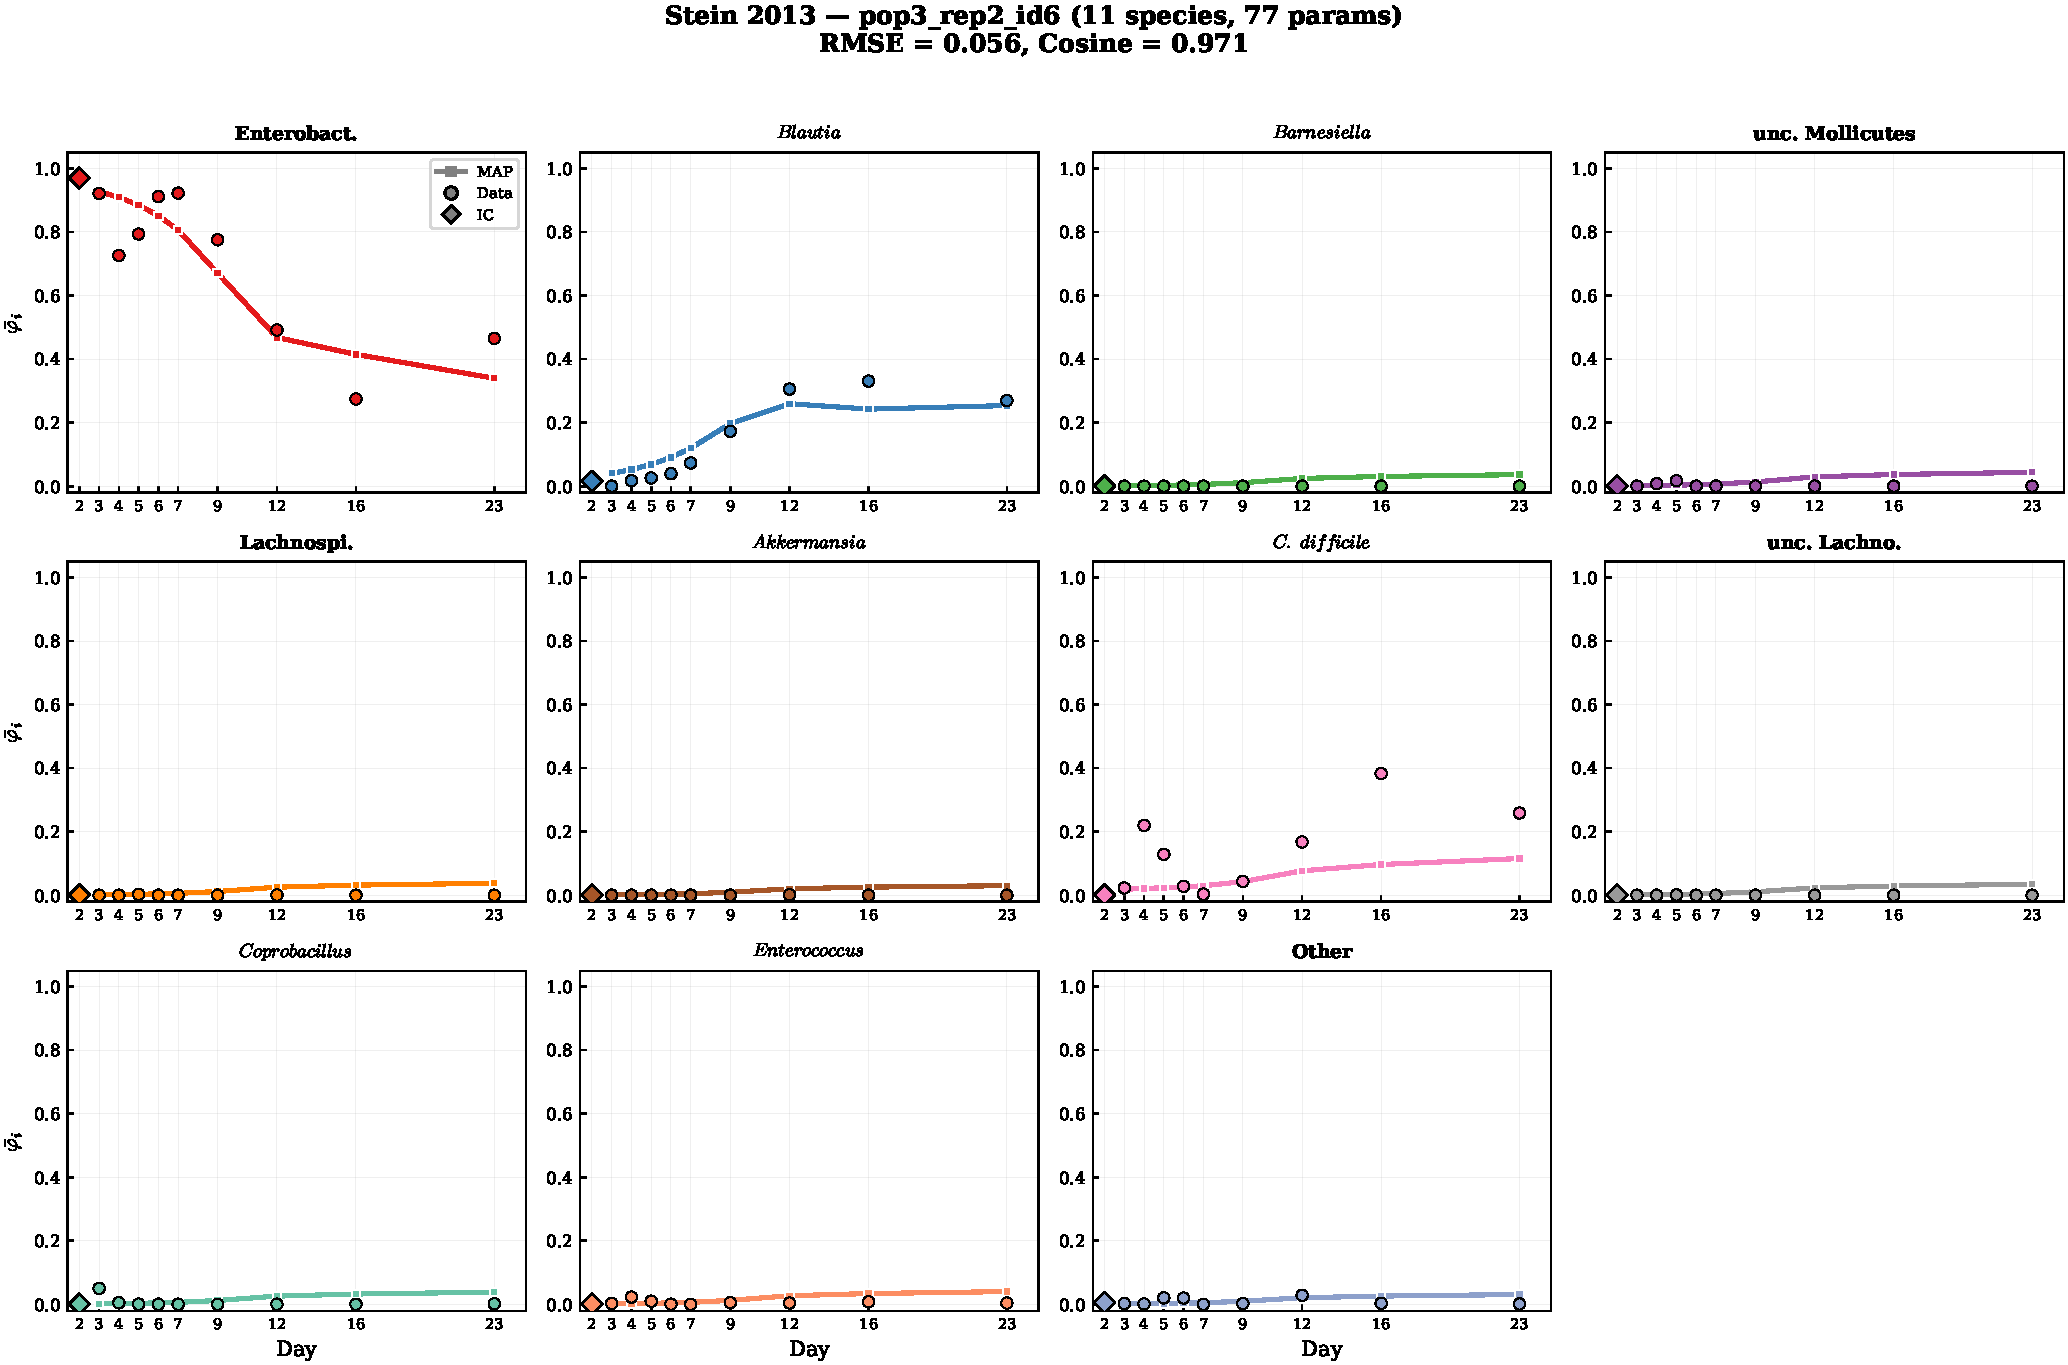
\includegraphics[width=\textwidth]{figures/fig_panels_pop3_rep2_id6.pdf}
\caption{Species-resolved fit for pop3\_rep2 (RMSE = 0.056). Squares:
MAP prediction. Circles: observed data. Diamond: initial condition (Day~2).
The model captures the Enterobacteriaceae decline, Blautia and
\textit{C.\ difficile} emergence, and late Mollicutes dominance.}
\label{fig:best_fit}
\end{figure}

\subsection{Cross-domain transferability}

To assess generalizability beyond gut microbiomes, we applied the identical
Hamilton ODE framework to the 6-species oral biofilm dataset of Siddiqui
et al.\ (2021) \cite{siddiqui2021}. Without any structural modifications,
the model achieves RMSE = 0.086 (planktonic) and 0.097 (adherent),
demonstrating that the variational formulation captures fundamental
interspecies dynamics across biological domains.

% ================================================================
\section{Discussion}

\subsection{Why symmetric $A$ works}

The key insight is that the symmetric interaction matrix serves as
\textbf{structural regularization}. In the 77-dimensional parameter space,
the symmetry constraint halves the number of free interaction parameters
(66 vs.\ 121), dramatically reducing the posterior volume and improving
identifiability. This is analogous to the role of symmetry in physics:
energy conservation (via the variational principle) constrains the
dynamics to physically realizable trajectories, preventing overfitting
to noise in the data.

The fact that Hamilton ODE matches or exceeds gLV performance with fewer
parameters suggests that \textbf{the non-symmetric degrees of freedom in
gLV are largely fitting noise} rather than capturing genuine asymmetric
interactions. This is consistent with the observation that most
experimentally characterized microbial interactions (metabolic cross-feeding,
competitive exclusion, coaggregation) have approximately symmetric effects
on the interacting partners.

\subsection{Compositional data advantage}

The Hamilton ODE natively produces compositional output
($\sum \bar{\varphi}_i = 1$), eliminating the need for absolute biomass
quantification. This is practically significant because:
(i) total biomass normalization via universal qPCR introduces systematic
error; (ii) many sequencing-based methods (16S amplicon, metagenomics)
only provide relative abundances; and (iii) the compositional constraint
prevents divergent trajectories that plague unconstrained gLV.

\subsection{Limitations}

\begin{enumerate}
\item \textbf{Time-invariant interactions}: The current formulation
assumes constant $A_{ij}$, which fails for acute perturbations
(clindamycin) and oscillatory dynamics (pop2). Incorporating
time-varying $A(t)$ or explicit perturbation susceptibility parameters
$s_i$ (as in gLV extensions) is a natural next step.

\item \textbf{Observable degeneracy}: Only $\bar{\varphi}_i = \varphi_i
\cdot \psi_i$ is measurable, leaving the $\varphi$--$\psi$ decomposition
under-determined. While the variational structure constrains this
decomposition, some parameter trade-offs persist.

\item \textbf{Computational cost}: The 77-dimensional TMCMC requires
$\sim$2--4 hours on GPU (NVIDIA RTX 4090, 5{,}000 particles). This is
comparable to gLV inference but scales as $O(N^2)$ in the number of
Newton iterations per ODE step.
\end{enumerate}

\subsection{Outlook}

The $N$-species generalized Hamilton ODE solver developed here is freely
available and applicable to any multispecies community with time-resolved
compositional data. Promising extensions include: (i) time-varying
interactions for antibiotic response modeling; (ii) spatial coupling
via finite element methods for biofilm mechanics; and (iii) integration
with neural network surrogates (DeepONet) for real-time inference.

% ================================================================
\section*{Data and code availability}

The Stein et al.\ (2013) dataset is available from PLoS Computational
Biology (Supplementary Table~S1). The Hamilton ODE solver and TMCMC
pipeline are available at \url{https://github.com/keisuke58/Tmcmc202601}.

% ================================================================
\section*{References}

\begin{thebibliography}{99}

\bibitem{stein2013}
Stein RR, Bucci V, Toussaint NC, et al.
Ecological modeling from time-series inference: insight into dynamics
and stability of intestinal microbiota.
\textit{PLoS Comput Biol} 9(12):e1003388, 2013.

\bibitem{bucci2016}
Bucci V, Tzen B, Li N, et al.
MDSINE: Microbial Dynamical Systems INference Engine for microbiome
time-series analyses.
\textit{Genome Biol} 17:121, 2016.

\bibitem{gerber2014}
Joseph TA, Shenhav L, Xavier JB, Halperin E, Pe'er I.
Compositional Lotka-Volterra describes microbial dynamics in the simplex.
\textit{PLoS Comput Biol} 16(5):e1007917, 2020.

\bibitem{buffie2015}
Buffie CG, Bucci V, Stein RR, et al.
Precision microbiome reconstitution restores bile acid mediated resistance
to \textit{Clostridium difficile}.
\textit{Nature} 517:205--208, 2015.

\bibitem{ching2007}
Ching J, Chen YC.
Transitional Markov Chain Monte Carlo method for Bayesian model updating,
model class selection, and model averaging.
\textit{J Eng Mech} 133(7):816--832, 2007.

\bibitem{klempt2024}
Klempt D, Nishioka K, Nackenhorst U.
Hamilton formulation for multispecies biofilm mechanics.
\textit{(In preparation)}, 2024.

\bibitem{siddiqui2021}
Siddiqui DA, Fidai AB, Natarajan SG, Rodrigues DC.
Succession of oral bacterial colonizers on dental implant materials.
\textit{Dental Materials} 38(2):384--396, 2022.

\bibitem{nishioka2026_oral}
Nishioka K, Klempt D, Nackenhorst U.
Multiscale Bayesian inference of oral biofilm mechanics via Hamilton ODE.
\textit{(In preparation)}, 2026.

\end{thebibliography}

\end{document}
